% !TEX root = ../main.tex

\subsection{ATLAS Humanoid Robot}

\ldots Humanoid by Boston Dynamics (see Fig. \ref{Fig:AtlasDoorFinals}), \ldots, BDI control modes (aka ``behaviors"), see Fig. \ref{Fig:ControlModeTS}.

\begin{figure}[t]
\centering
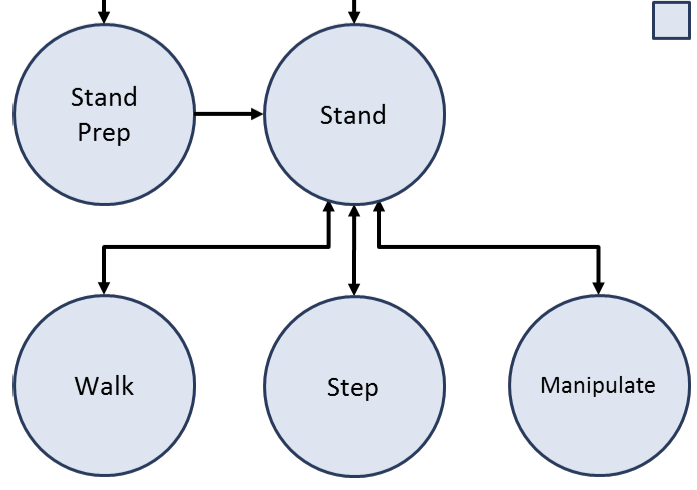
\includegraphics[width=0.99\columnwidth,clip]{./img/control_modes_ts.png}
\caption{\ldots
	\todo[inline, caption = {Create a simple control mode TS figure}]{Placeholder! Create simple control mode TS figure (flat).}
}
\label{Fig:ControlModeTS}
%\vspace{-3 pt}
\end{figure}

\subsection{Team ViGIR's Approach}

\subsubsection{Something}  \ldots \cite{ROS2009ICRA, ROS} \ldots Briefly touch on our software approach \cite{TeamViGIR2014JFR}, especially control modes and templates \cite{Alberto2014Humanoids}. Just enough for the ``High-level Control" subsection and the experimental demos to make sense.

Define \emph{system} as ATLAS plus Team ViGIR software.

\subsubsection{High-level Control} 

\ldots SMACH \cite{SMACH2010RAM}, Behavior control \cite{Philipp2013Bsc, Philipp2015Msc} FlexBE\footnote{\scriptsize{\url{https://github.com/team-vigir/flexbe_behavior_engine}}}
, GUI\footnote{\scriptsize{\url{https://github.com/team-vigir/flexbe_chrome_app}}}
, behaviors and states\footnote{\scriptsize{\url{https://github.com/team-vigir/vigir_behaviors}}}.

Some incomplete notes from Philipp's work. Not sure yet how much detail is needed here.
\todo[inline, caption = {Make FlexBE and Synthesis notation consistent}]{Philipp's definitions differ slightly from the synthesis literature. Ensure that we end up with consistent notation.}
\begin{itemize}
	\item A primitive $p \in P$ is any atomic capability of the robot.
	\item A state $s \in S$ interfaces functionality with behaviors, where the set of all state implementations $S$ includes states based on primitives $S_p \subseteq S$. Each state defines outcomes $s_{Oc}$ and execution of a state is terminated by returning one outcome matching the result of execution $oc \in s_{Oc}$.
	\item A state machine SM composes a set of states $S_{SM}$, where each state $s(i) \in S_{SM}$ is the instantiation of a state implementation $s \in S$.
	\item Each state machine SM defines userdata $D_{SM}$
	\item A behavior B is implemented by its state machine $B_{SM}$.
\end{itemize}

Example: Fig. \ref{Fig:FlexBESM} \ldots designed manually by Team ViGIR developers using the FlexBE Editor (graphical user interface).

\begin{figure}[t]
\centering
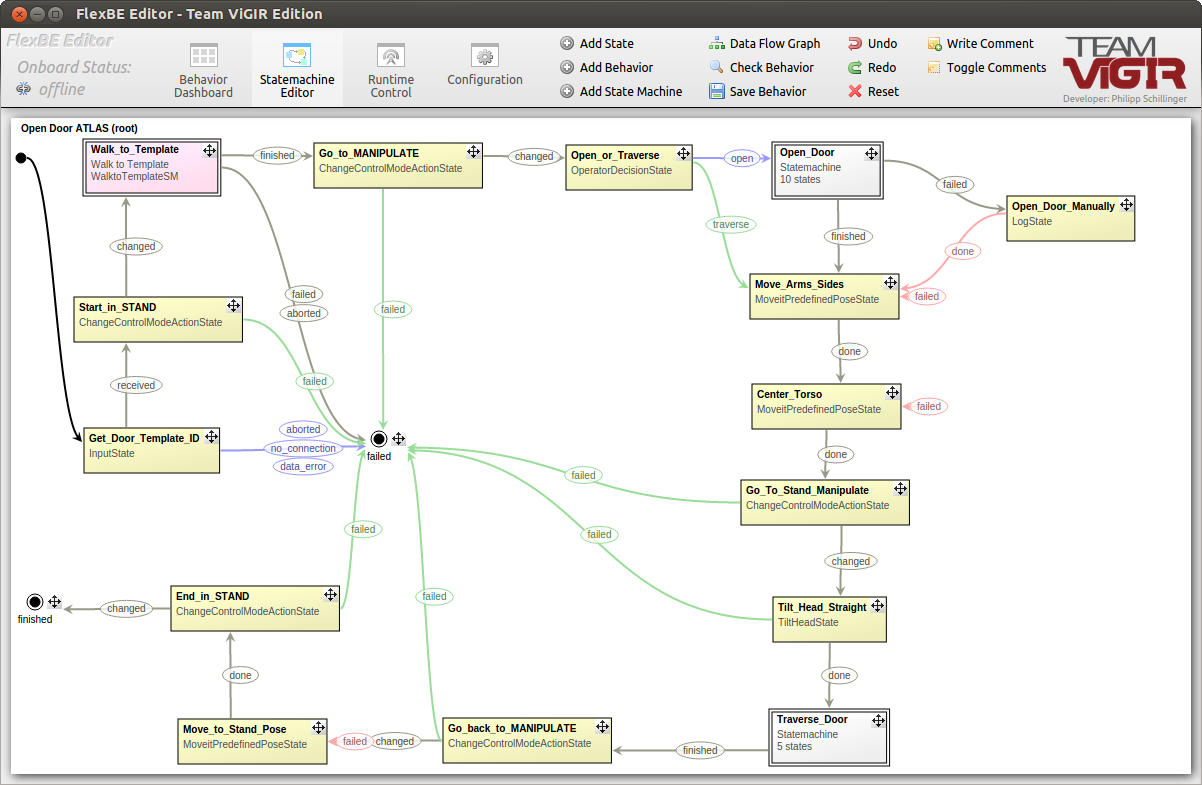
\includegraphics[width=0.99\columnwidth,clip]{./img/behavior_open_door.png}
\caption{A high-level behavior for carrying out the DRC Finals' ``Door" task.
The initial state is indicated by the black arrow originating from the top left.
This state machine has two outcomes, ``finished" (bottom left) and ``failed" (center).
This is a hierarchical state machine.
Yellow states are primitives, gray states are state machines, and purple states are other high-level behaviors embedded in this one.
}
\label{Fig:FlexBESM}
\end{figure}

\subsection{Linear Temporal Logic and Reactive LTL Synthesis}

\ldots Atomic propositions, LTL, environment vs system, etc.

GR(1) formulas $\varphi$ have an assume-guarantee structure between the environment ($e$) and the system ($s$):
%$\varphi = (\varphi_e \Rightarrow \varphi_s)$, where:
%$$\varphi_e = \varphi_e^i \wedge \varphi_e^t \wedge \varphi_e^g, \; \varphi_s = \varphi_s^i \wedge \varphi_s^t \wedge \varphi_s^g,$$
\begin{equation}\label{GR1Formula}
\begin{split}
	\varphi &= (\varphi_e \Rightarrow \varphi_s),\\
	\varphi_e &= \varphi_e^i \wedge \varphi_e^t \wedge \varphi_e^g,\\
	\varphi_s &= \varphi_s^i \wedge \varphi_s^t \wedge \varphi_s^g,
\end{split}
\end{equation}
where the superscript $i$ denotes initial conditions, $t$ safety assumptions/requirements, and $g$ liveness assumptions/requirements (goals) for the environment and the system, respectively. 

GR(1) Synthesis \cite{piterman_06} \ldots

% END